\documentclass[12pt]{article}
\usepackage{amsmath, amssymb, graphicx, hyperref}
\usepackage{indentfirst}
\title{Plasma Mirrors}
\author{Harikesh}
\date{\today}

\newenvironment{changemargin}[2]{%
\begin{list}{}{%
\setlength{\topsep}{0pt}%
\setlength{\leftmargin}{#1}%
\setlength{\rightmargin}{#2}%
\setlength{\listparindent}{\parindent}%
\setlength{\itemindent}{\parindent}%
\setlength{\parsep}{\parskip}%
}%
\item[]}{\end{list}}
\begin{document}
\begin{titlepage}
    \begin{changemargin}{-2cm}{-2cm}
        \begin{figure}
            
\includegraphics[width=5cm, height=5cm]{logo.png}
            \centering
        \end{figure}
        \begin{center}
            \textbf{\Large{Department of Physics, IIT Delhi}}\\
            \vspace*{1cm}
            \textbf{\Large{Course Code : PYD561}}\\
            \vspace*{0.2cm}
            \textbf{\Large {Semester - III, 2022-23}}\\
            \vspace*{1cm}
            \textbf{\LARGE{Plasma Mirrors}}\\
            \vspace*{1cm}
            \textbf{\Large{Kulwinder Kaur (2021PHS7190)}}\\
            \vspace*{0.2cm}
            \textbf{\Large {Harikesh Kushwaha (2021PHS7181)}}\\
            \vspace*{1cm}
            \textbf{\Large {Adviser: Prof. Vikrant Saxena}}\\
            \vspace*{2cm}
        \end{center}
        \begin{flushleft}


            \textbf{Signature of student 1: \ldots \ldots \ldots}\\
            \vspace*{1cm}
            \textbf{Signature of student 2: \ldots \ldots \ldots}
            \hspace*{3cm}
            \textbf{Signature of the adviser: \ldots \ldots \ldots}
        \end{flushleft}
    \end{changemargin}
\end{titlepage}
\newpage
\begin{changemargin}{-3cm}{-3cm}
    \section{Introduction And Motivation}
    The generation of harmonics by interaction of an ultrashort high intensity laser pulse with a step boundary of a overdense plasma layer is studied at various intensities. For this, fully relativistic particle-in-cell (PIC) simulations are performed using \textit{epoch}.

    When a laser pulse is incident upon plasma, it reflects if the density of plasma is large enough, forming a plasma mirror (PM). Upon reflection from the plasma the laser field drives relativistic oscillation of the PM surface due to pondermotive force that induces a periodic temporal compression of the reflected field through the Doppler effect. These oscillations results in generation of high harmonics of the incident laser frequency.\cite{lichters}

    The idea is to generate high harmonics which can then be focused to achieve light intensities higher than currently available intensity ($I \approx 10^{22}$ $W.cm^{-2}$). Light with these high intensities can be used to investigate light-matter interation in regimes barely explored in lab.\cite{henri}


    \section{Methodology}
    The simulation uses \textit{epoch}, a parallised, second order and fully relativistic implementation of particle in cell (PIC) algorithm.\cite{epoch} Though \textit{epoch} is implemented in 3D, the current simulation is performed in 1D3V only.
    % which implementats a fully relativistic particle in cell (PIC) algorithm.
    \subsection{PIC Algorithm}
    In plasma physics, the PIC method is a numerical approach that simulates a collection
    of charged particles that interact via external and self-induced electromagnetic fields. A
    spatial grid is used to describe the field while the particles move in the continuous space. The field and the particle motion are solved concurrently. In this case the simulation
    requires less amount of work, since each particle only interacts with the grid points of
    the cell where it is located.\cite{suciu}

    In PIC, the plasma is represented by collection of particles, macro particle, with same charge to mass ratio. The system is discretised parallel to the boundaries forming a grid (mesh). The particles are free to move anywhere inside the system boundaries, however, the continuous electromagnetic field is replaced by discrete values assigned only to the mesh points.

    % \newpage
    % \noindent
    The arrangement of the fields is called the Yee cell.
    Since the charge density is defined on the corners, the central difference places the electric fields at the edges. Meanwhile, the magnetic fields are located on the face. After the initial condition is given, PIC start by calculating the charge density ($\rho$) at grid points from nearby charged
    particles. The charge of each particle is distributed among the grid points using a weighting algorithm. Usually, a bilinear interpolation is used where the charge on the grid is determined using the subarea of the opposite vertex.
    % \begin{minipage}{0.6\textwidth}\raggedright
    %     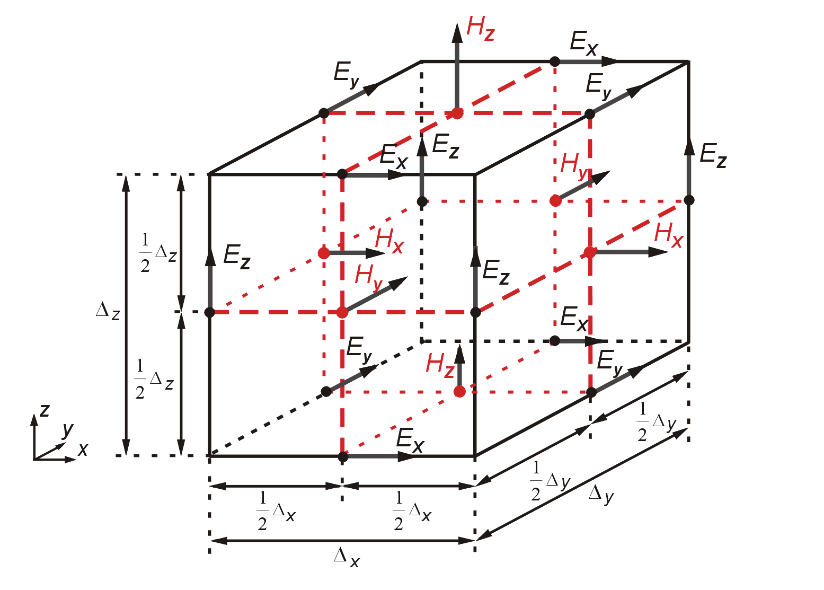
\includegraphics[height=7cm, width=7cm]{yee.png}
    % \end{minipage}
    % \begin{minipage}{0.35\textwidth}\raggedright
    %     The arrangement of the fields is called the Yee grid.
    %     Since the charge density is defined on the corners, the central difference places the electric fields at the edges. Meanwhile, the magnetic fields are located on the face.
    % \end{minipage}

    % \noindent
    % \begin{minipage}{0.55\textwidth}\raggedleft
    %     After the initial condition is given, PIC start by calculating the charge density ($\rho$) at grid points from nearby charged
    %     particles. The charge of each particle is distributed among the grid points using a weighting algorithm. Usually, a bilinear interpolation is used where the charge on the grid is determined using the subarea of the opposite vertex.
    % \end{minipage}
    % \begin{minipage}{0.4\textwidth}\raggedleft
    %     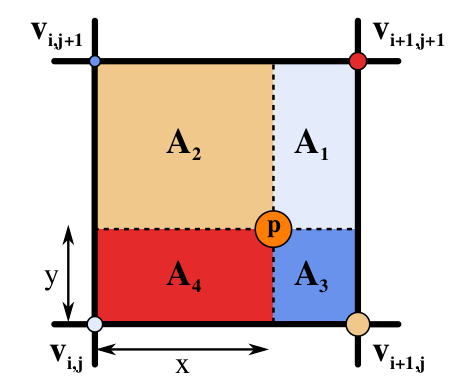
\includegraphics[height=5cm, width=5cm]{charge.png}
    % \end{minipage}
    \vspace*{0.5cm}

    Update of $\mathbf{E}$ and $\mathbf{B}$ is done by Yee algorithm. The advancement of $\mathbf{E}$ from step $n$ to $n+1$ is done via central differencing using $\mathbf{B}$ at $n+1/2$. While, the advancement of $\mathbf{B}$ from step $n-1/2$ to $n+1/2$ is done via central differencing using $\mathbf{E}$ and the current density ($\textbf{J}$) at step $n$. Finally, the updated electric and magnetic fields are used to forward velocity for step $n-1/2$ to $n+1/2$ and velocity at step $n+1/2$ is used to forward position for step $n$ to $n+1$. The charge and hence the current density is updated using this newly updated position which in turn updates magnetic field and the cycle continues. The fact that the velocity ($\mathbf{B}$) at half step is used to forward position ($\mathbf{E}$) at full step and vice versa makes this update rule leap-frog method.

    The velocity is updated with Boris method. First, a half-step acceleration is performed in the electric field direction, followed by full rotation in magnetic field and finally, another half-step acceleration is performed in the electric field direction.
    \subsection{Underdense and Overdense Plasma}
    Plasma frequency for plasma density $n_p$ is given by\cite{chen}
    \begin{equation}\label{plasma-frequency}
        \omega_p = \sqrt{\frac{n_p e^2}{\epsilon_0 m_e}}
    \end{equation}
    If the frequency of the incident laser pulse, $\omega_l$, is greater than the plasma frequency, the plasma is called underdense. In this case, the plasma is transparent to the laser pulse. On the other hand, if the frequency of the incident laser pulse is less than the plasma frequency, the plasma is called overdense. In this case, the laser can not penetrate the plasma deeply and is reflected back. The case $\omega_l = \omega_p$ corresponds to critical plasma and density in this case is called critical density $n_c$. Using Equation \hyperref[plasma-frequency]{1} gives;
    \begin{equation}\label{critical-density}
        n_c = \frac{\epsilon_0 m_e \omega_l^2}{e^2}
    \end{equation}
    % The skin depth of the plasma is given by
    % \begin{equation*}
    %     \delta = \frac{c}{\omega_p}
    % \end{equation*}
    \subsection{Laser Pulse}
    The simulation uses ultrashort laser pulses. An ultrashort laser emitts pulse with duration of the order of pico second. Defining the laser vector potential as $ a_0 = \frac{eE_0}{m w_l c}$, a laser is called relativistic if $a_0 \ge 1$. For a laser wavelength of $1 \mu m$ laser the intensity $1.4 \times10^{22}$  $W.m^{-2}$ corresponds to $a_0=1$.

    \subsection{Parameters for Simulation}
    The simulation box extends for $8 \lambda _l$ (from $-4 \lambda _l$ to $4 \lambda _l$), where $\lambda_l$ is the laser wavelength and has total 1000 cells. The plasma is placed at $x=0$ and with a thickess of $\lambda_l$. Number of particles per cell are 100. Initial temperature of electron is $50 \; eV$. The plasma density $n_p$ is defined in terms of the critical density $n_c$.

    The envelope of the incident laser field varies according to
    \begin{equation}\label{envelope}
        P(t)=
        \begin{cases}
             & \sin^2(\pi t/T) \text{ for } 0 \leq t \le T \\
             & 0         \;      \text{ otherwise }
        \end{cases}
    \end{equation}
    Where T is the pulse duration here taken as $T=20\tau$ with $\tau = 2\pi/\omega_l$ is the time of one laser cycle. The simulation is performed for $t=55\tau$.
    \section{Result and Discussion}
    \section{Current Status and Future Plan of Work}
    Simulation of harmonic generation in 1D using ultrashort intense laser pulse is performed. Future plan is to expand the Simulation to 2D and use focusing techniques to generate extreme intensity light beam.
    \section{Acknowledgement}
    We are very thankful to Prof. Vikrant Saxena for his support and valuable guidance.
    % \section{References}
    \begin{thebibliography}{9}
        \bibitem{lichters}
        R. Lichters Et al. Physics of Plasmas 3, pp. 3425-3437 (1996)

        \bibitem{henri}
        Henri Vincenti Phys. Rev. Lett. 123, 105001 (2019)

        \bibitem{epoch}
        Arber, T D Et al. Plasma Physics and Controlled Fusion 57 1-26 (2015)

        \bibitem{suciu}
        Alin Suciu Et al. 2020 15th Conference on Computer Science and Information Systems (FedCSIS), pp.381-385, 2020

        \bibitem{chen}
        Francis F. Chen
        Introduction to Plasma Physics and Controlled Fusion $3^{rd}$ Ed.

    \end{thebibliography}

\end{changemargin}
\end{document}